\documentclass[12pt]{article}

\usepackage{pictex}
\usepackage{multirow}
\usepackage{color}
\usepackage[pdftex]{graphicx}
\usepackage{fancyhdr}
\usepackage[portuguese]{babel}
\usepackage[utf8]{inputenc}
\usepackage{xcolor,colortbl}
\usepackage{placeins}
\usepackage{verbatim}
\usepackage{geometry}
\usepackage{lscape}
\usepackage{listings}
\usepackage{color}
\usepackage{times}
\usepackage{afterpage}
\usepackage{hyperref}



\definecolor{dkgreen}{rgb}{0,0.6,0}
\definecolor{gray}{rgb}{0.5,0.5,0.5}
\definecolor{mauve}{rgb}{0.58,0,0.82}

\lstset{frame=tb,
  language=Java,
  aboveskip=3mm,
  belowskip=3mm,
  showstringspaces=false,
  columns=flexible,
  basicstyle={\small\ttfamily},
  numbers=none,
  numberstyle=\tiny\color{gray},
  keywordstyle=\color{blue},
  commentstyle=\color{dkgreen},
  stringstyle=\color{mauve},
  breaklines=true,
  breakatwhitespace=true,
  tabsize=3
}

\newcommand{\HRule}{\rule{\linewidth}{0.2mm}}


 \geometry{
 total={210mm,297mm},
 left=30mm,
 right=30mm,
 top=30mm,
 bottom=30mm,
 }
 
 \pagestyle{fancy}
\fancyhf{}
\lhead{\footnotesize Architecture and Design of Software para Web dashboard para o git}
\rhead{\footnotesize 14 de Outubro de 2016}
\lfoot{}
\cfoot{\footnotesize Página \thepage}
\rfoot{}
 
 
 
\begin{document} 
\begin{titlepage}
\begin{center}

\textsc{\footnotesize Universidade de Coimbra }\\[0.1cm]
\textsc{\footnotesize Faculdade de Ciências e Tecnologias}  \\[0.1cm]
\textsc{\footnotesize Departamento de Engenharia Informática }\\[0.2cm]
\textsc{\footnotesize Engenharia de Software }\\[2cm]




{\Large \bfseries Architecture and Design of Software\\[1.5cm]

\textsc{\normalsize Version 0.4}\\[.2cm]
\textsc{\normalsize Web Dashboard para o Git}\\[2cm]
\textsc{\fontsize{2cm}{2.5cm}\selectfont EdgeSoft}\\[5cm]


\small
André Duarte \hfill 2014214845\\ 
Diana Pereira \hfill 2013150712\\
Gonçalo Pinto \hfill 2014202176\\
Henrique Pereira \hfill 2011154576\\
João Costa \hfill 2013144034\\
João Ferreiro \hfill 2014197760\\
Joel Pires \hfill 2014195242\\



\begin{minipage}{0\textwidth}
\begin{flushright} \large
\end{flushright}
\end{minipage}

\vfill
{\normalsize 14 de Outubro de 2016}
}

\end{center}
\end{titlepage}


\pagebreak

\tableofcontents

\pagebreak

\section{ \textsc{Tabela de Revisões}}


\begin{center}
\begin{tabular}{ | m{1cm} | m{5cm}| m{3cm} | m{5cm} | } 
\hline
Versão & Data & Autor & Descrição \\ 
\hline
0.4 & 14/10/2016 & Joel \& Henrique & Revisão do conteúdo dos diagramas\\ 
\hline
0.3 & 14/10/2016 & Joel \& Henrique & Revisão do conteúdo dos diagramas\\ 
\hline
0.2 & 13/10/2016 & Joel \& Henrique & Criação dos diagramas\\ 
\hline
0.1 & 13/10/2016 & Joel \& Henrique & Estrutura inicial do documento\\ 
\hline
\end{tabular}
\end{center}




\pagebreak

\section{ \textsc{Arquitetura e Design do Software}}
\subsection{ \textsc{Padrão de Arquitetura}}
O padrão arquitetural escolhido foi o \textbf{MVC (Model View 	Controller)} uma vez que é o mais adequado e usado para aplicações web. A própria framework escolhida para o desenvolvimento da aplicação (Meteor) facilmente se adapta a este modelo. 
Esta arquitetura permite-nos dividir um grande problema em vários problemas menores e de menor complexidade, excelente para aplicar modelo de processos adotado (SCRUM). O facto de haver uma divisão entre camadas faz com que possamos trabalhar independentemente em diferentes partes da aplicação sem afetar o “workflow” (aspeto relevante quando uma equipa tem diferentes “skill sets”). O reaproveitamento, limpeza, alteração e manutenção do código também fica facilitado.


\vspace{5mm}

\begin{figure}[h!]
	\centering 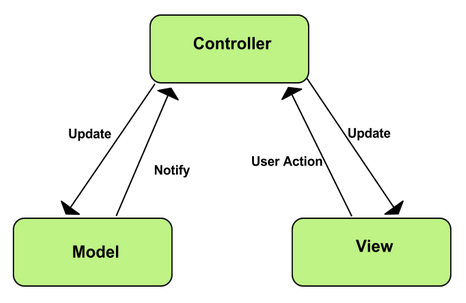
\includegraphics[width=12cm]{public/Architecture and Design of Software_1.png}
	\caption{Diagrama do MVC}
\end{figure}

\vspace{5mm}


\pagebreak
\subsection{ \textsc{Diagrama da Arquitetura de Alto Nível}}


\vspace{5mm}

\begin{figure}[h!]
	\centering 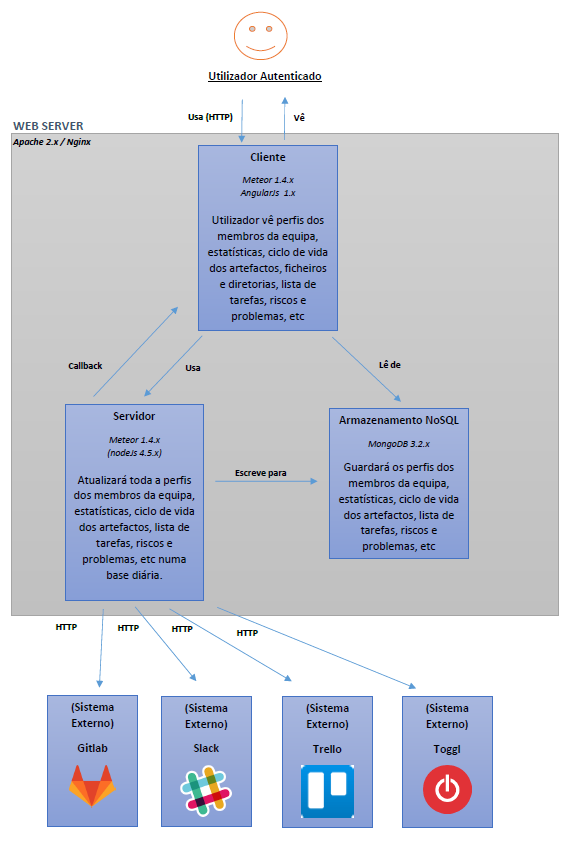
\includegraphics[width=12cm]{public/Architecture and Design of Software_2.png}
	\caption{Diagrama da Arquitetura de Alto Nível}
\end{figure}

\subsection{ \textsc{Design Detalhado}}
\subsubsection{ \textsc{Servidor}}
\begin{figure}[h!]
	\centering 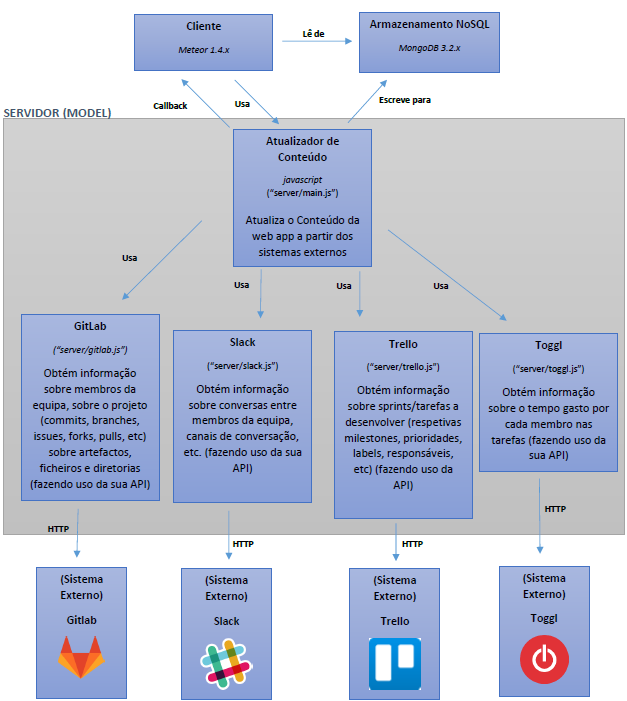
\includegraphics[width=12cm]{public/Architecture and Design of Software_3.png}
	\caption{Design Detalhado do Servidor}
\end{figure}

\pagebreak


\subsubsection{ \textsc{Cliente}}
\begin{figure}[h!]
	\centering 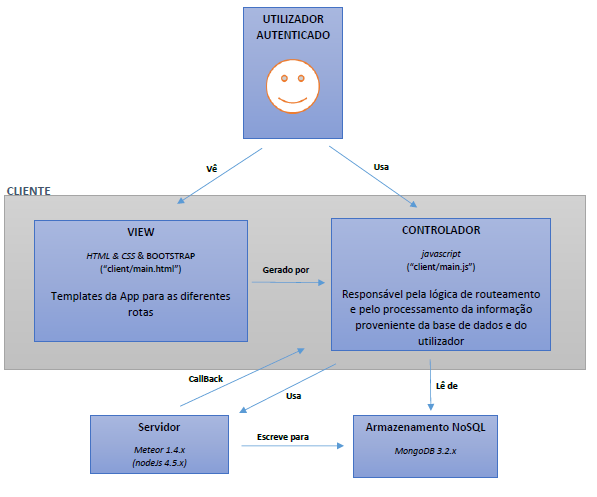
\includegraphics[width=9cm]{public/Architecture and Design of Software_4.png}
	\caption{Design Detalhado do Cliente}
\end{figure}

\vspace{5mm}

\subsubsection{ \textsc{Base de Dados}}
\begin{figure}[h!]
	\centering 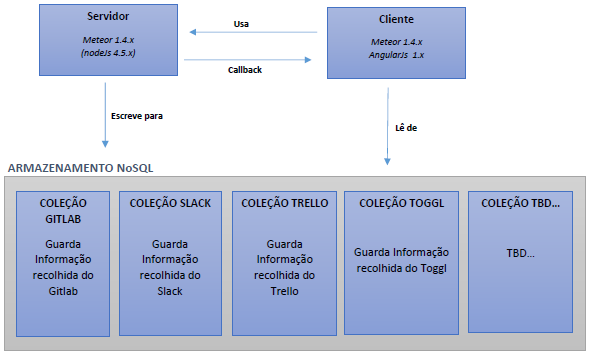
\includegraphics[width=9cm]{public/Architecture and Design of Software_5.png}
	\caption{Design Detalhado da Base de Dados}
\end{figure}


\pagebreak

\subsection{ \textsc{Tecnologias Usadas}}

\textbf{Sistemas Operativos:}
\begin{itemize}
\item Linux
\end{itemize}
\hfill \linebreak

\textbf{Tecnologias:}
\begin{itemize}
\item Meteor
\item nodeJS
\item Angularjs
\item MongoDB
\item Bootstrap
\item OAuth2
\item Apache/Nginx
\end{itemize}
\hfill \linebreak

\textbf{Linguagens:}
\begin{itemize}
\item Javascript
\item HTML \& CSS
\end{itemize}
\hfill \linebreak

\textbf{Interfaces:}
\begin{itemize}
\item Http
\item REST
\item JSON
\end{itemize}
\hfill \linebreak

\textbf{API’S:}
\begin{itemize}
\item Slack
\item Trello
\item Gitlab
\item Toggl
\end{itemize}
\hfill \linebreak

\pagebreak

\end{document}



















